\documentclass[a4paper]{article}

\usepackage{amsmath, blindtext, float, graphicx, hyperref}
\graphicspath{ {./images/} }
\title{Task A3: Exploring Data using Python and Plotly}
\author{Shubham Gupta \\ A0225160U}

\begin{document}
\maketitle
\section{Introduction}
\begin{itemize}
    \item For this task, we aim to explore the \href{https://github.com/rfordatascience/tidytuesday/tree/master/data/2022/2022-01-18}{Chocolate} dataset. 
    \item Through visualizations, we aim to answer a few questions.
    \item You can access the notebook by launching it in binder \href{https://mybinder.org/v2/gh/goodhamgupta/cs5346_task_A3/HEAD?labpath=A0225160U_A3.ipynb}{here}
    \item Incase you want to setup the notebook locally, the repository is available \href{https://github.com/goodhamgupta/cs5346_task_A3}{here}. 
\end{itemize}

\section{Implementation}
\subsection{Q1: Who makes the best chocolate with Ecudorian beans?}
\begin{itemize}
    \item In this visualization, we aim to check which countries make the best chocolate from Ecudatorian beans. The scoring is done based on the 'rating' of beans produced by each company.
    \item The country is identified by the location in of the company. In the visualization, we show the top 10 countries based on the number of ratings we have for each country.
    \item The visualization consists of a \textbf{Horizontal Violin Plot}. We choose this plot to demonstrate the range of ratings for the given to the chocolate made in the countries.
    \item The visualization is plotted for all breeds, and has a color coding signifying the "Coat Length" of each dog breed.
    \item The following visual encoding is used:
    \begin{itemize}
        \item The x-axis represents Rating, which is a ordinal attribute with the range between 1 to 5. Since rating values can never be negative, we use a "Horizontal Violin Plot".
        \item The y-axis represents the Country, which is a categorical attribute.
        \item Colors are used as "Channels", to denote the rating distributions for different countries.
    \end{itemize}
    \begin{figure}[H]
        \centering
        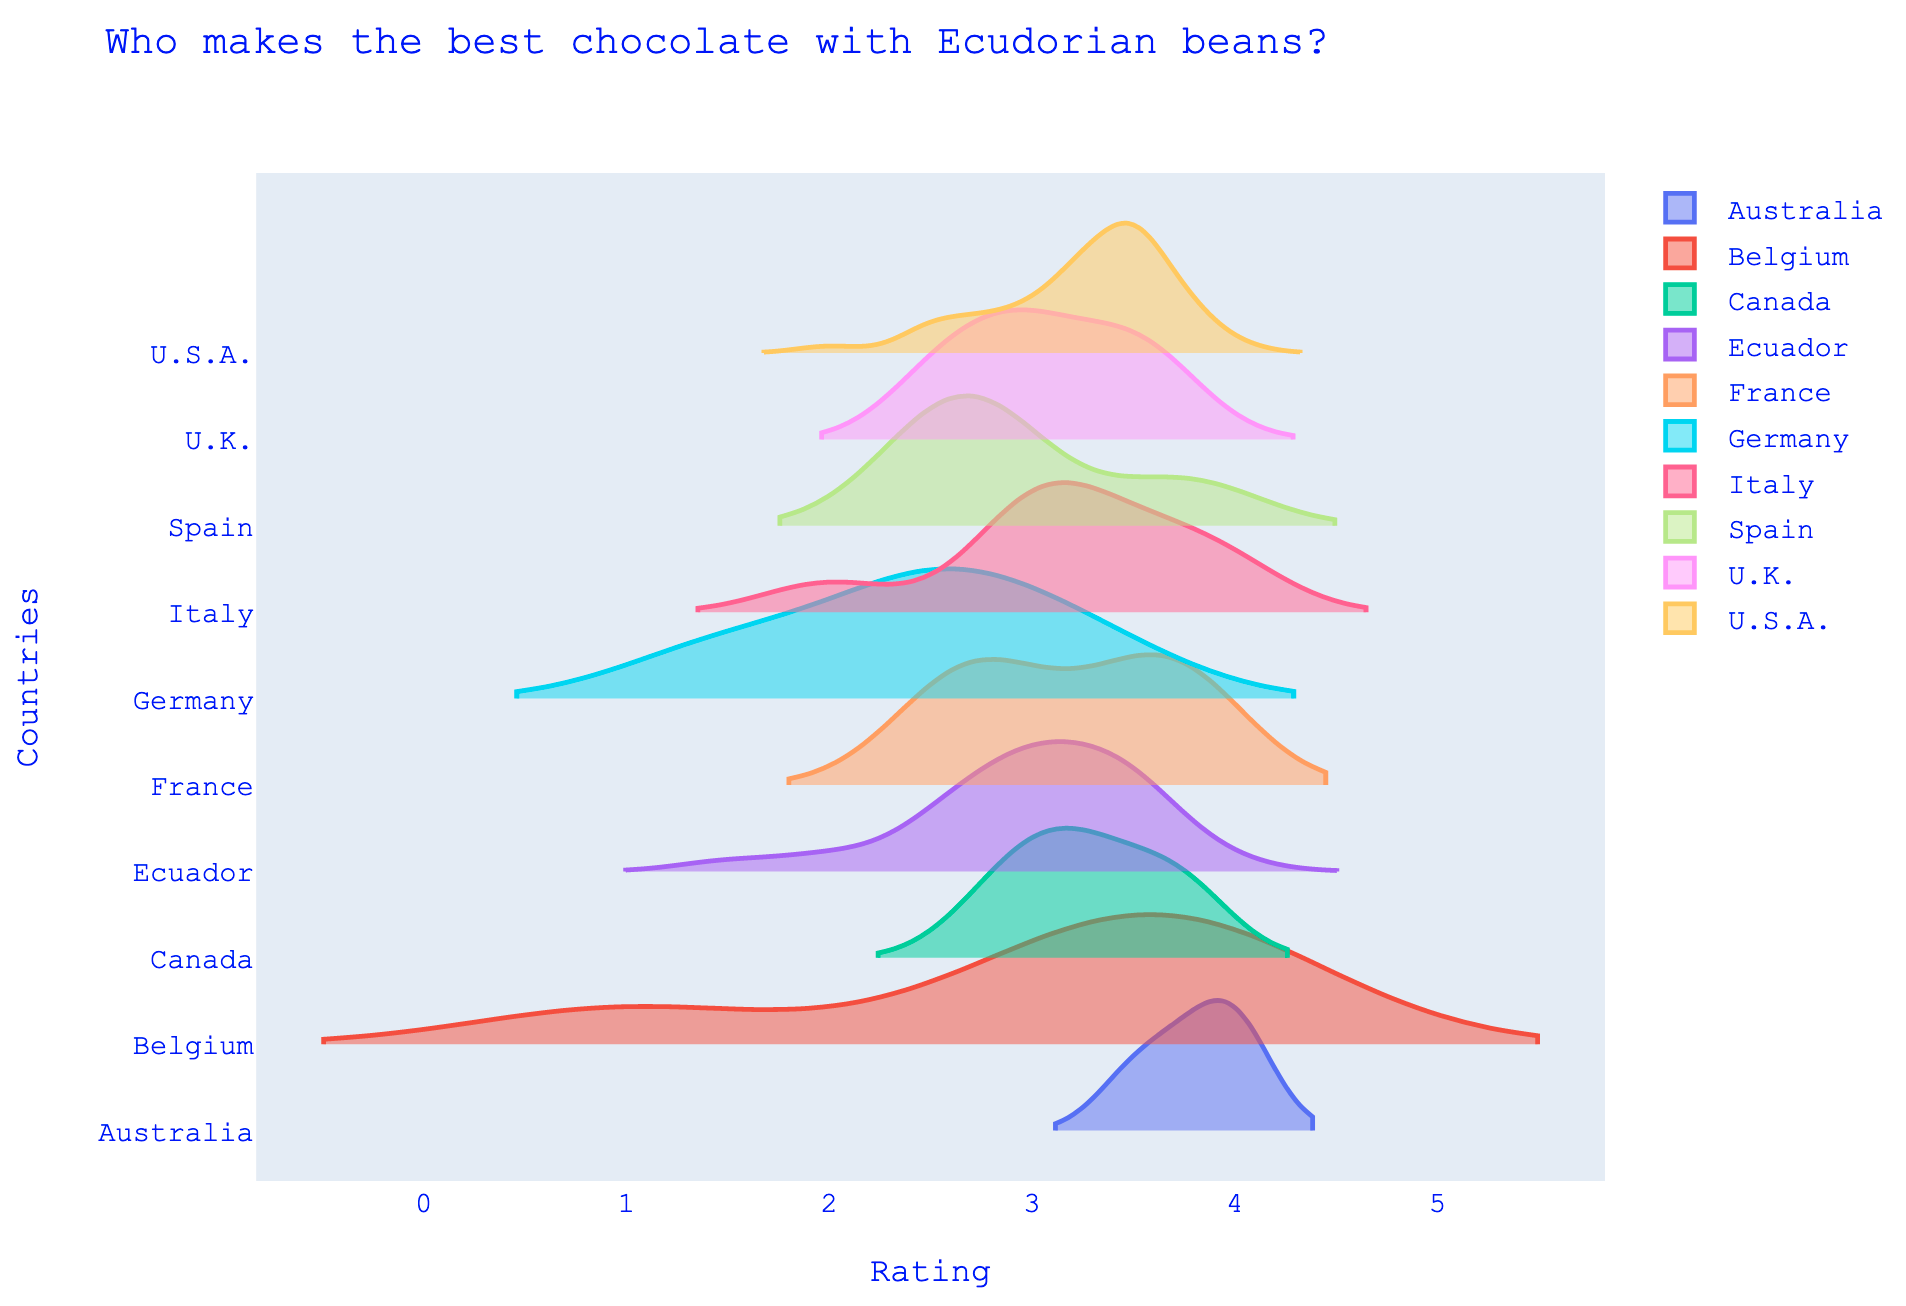
\includegraphics[width=1.0\textwidth]{violin}
        \caption{Who makes the best chocolate with Ecudorian beans?}
        \label{fig:violin}
    \end{figure}
    \item From the visualization, we see that the maximum rating for is 4 for the countries Belgium, Ecuador, USA and Italy, with Australia having the best ratings. 
\end{itemize}

\subsection{Q2: What words are used to describe chocolates?}
\begin{itemize}
    \item In this visualization, we aim to see the distribution of words used to describe chocolates. We compare the words used with the rating given for each chocolate.
    \item We use a \textbf{Box Plot} here, and only show the top 10 words as there are a total of 2455 unique words.
    \item The following visual encoding is used:
    \begin{itemize}
        \item The x-axis represents Rating, which is a ordinal attribute with the range between 1 to 5. 
        \item The y-axis represents Characteristic, which is the "word" used to describe the chocolate. This is a categorical variable.
        \item Colors are used as "Channels", to denote the ratings distributions for different words.
    \end{itemize}
    \begin{figure}[H]
        \centering
        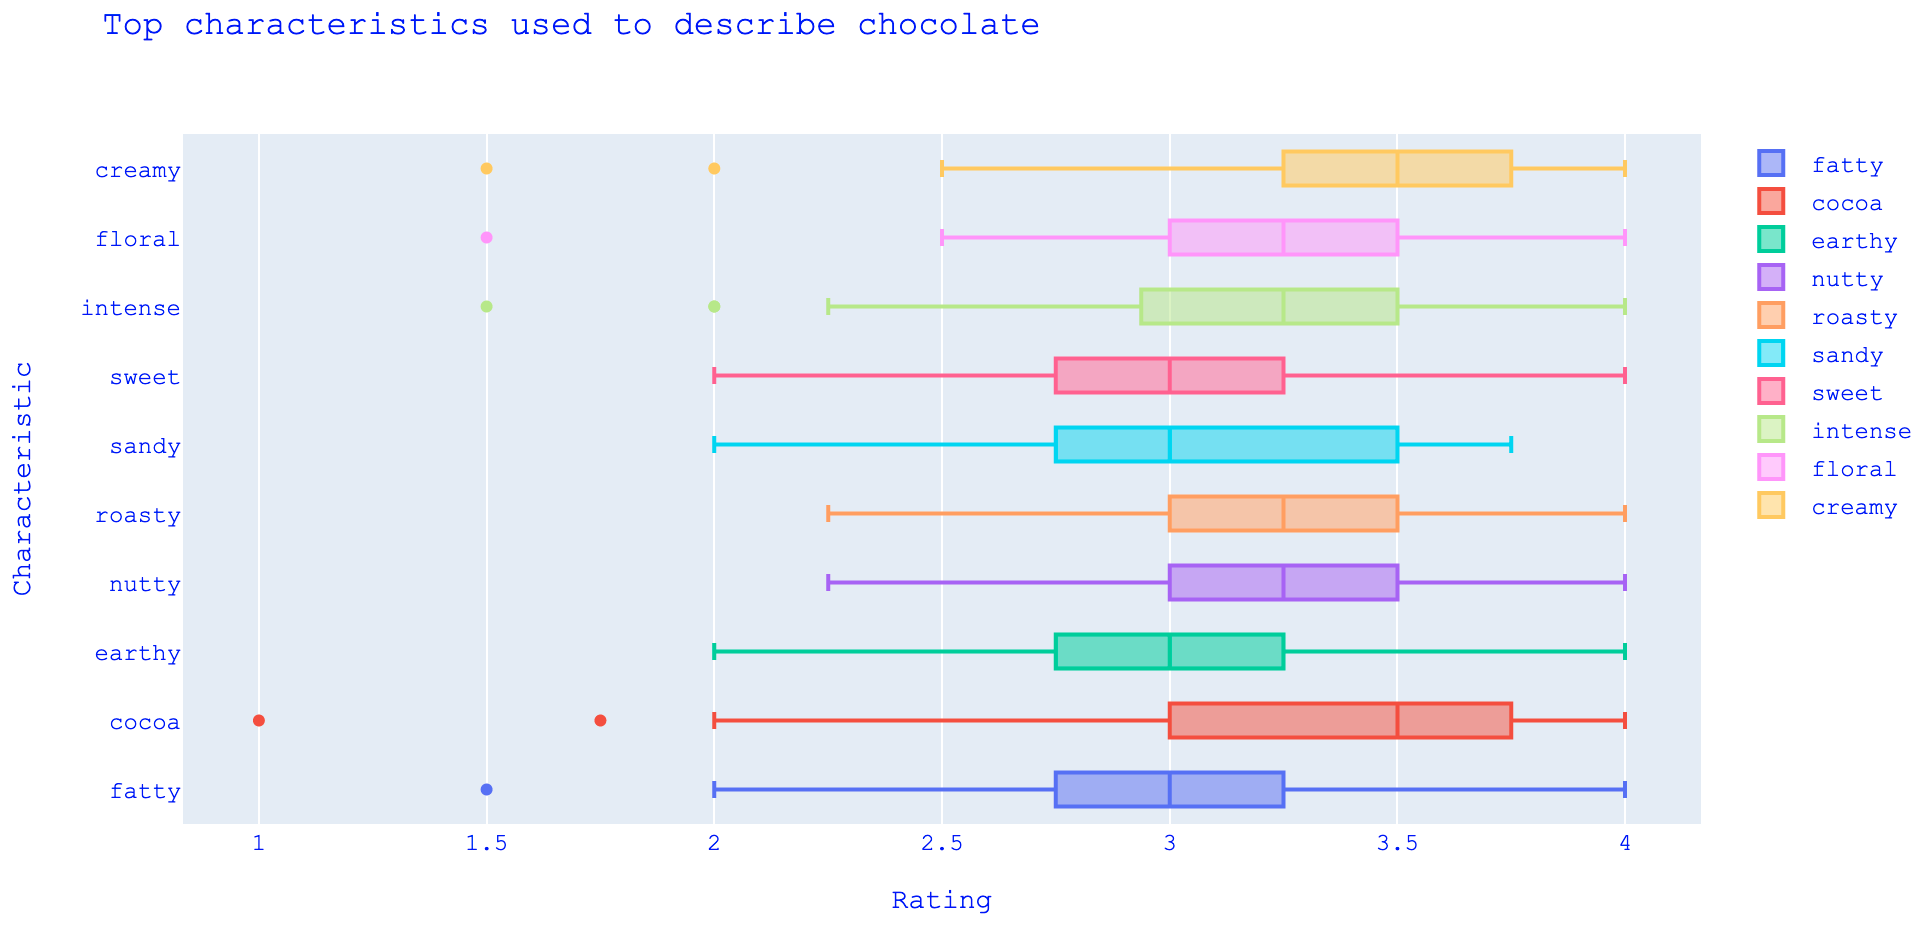
\includegraphics[width=1.0\textwidth]{box}
        \caption{What words are used to describe chocolates?}
        \label{fig:box}
    \end{figure}
    \item We see that "cocoa" and "creamy" are the words used to describe highly rated chocolates. Manufacturers should create chocolates with these two ingredients to have the best ratings!
\end{itemize}

\subsection{Q3: Dark Chocolate: Where does it come from and where does it go?}
\begin{itemize}
    \item For this visualization, we aim to visualize the movement of dark chocolate from the source to the destination country.
    \item By definition, we select only choclates that have a cocoa percentage of above 85\% as "Dark Chocolate". Note that similar to the previous question, the "destination" country is decided by the location of the "company" that produces the chocolate.
    \item We also preprocess the dataset to label encode both the source and the destination countries.
    \item We use a \textbf{Sankey Diagram} for the visualization, demonstrating the flow of dark chocolate from one region to another.
    \item The following visual encoding is used:
    \begin{itemize}
        \item The y-axis represents "Countries", which is a categorical variable. We use a dual y-axis for this plot.
        \item The "incoming flow count" and "outgoing flow count" are quantitative values.
        \item "Links" via lines are used to demonstrate the movement between a source and a destination country. For each link, "Color" is used as a channel.
        \item "Size" is used as a channel, to demonstrate the number of imports/exports for a given country. Larger the number, larger is the size of the "country" on the graph.
    \end{itemize}
    \begin{figure}[H]
        \centering
        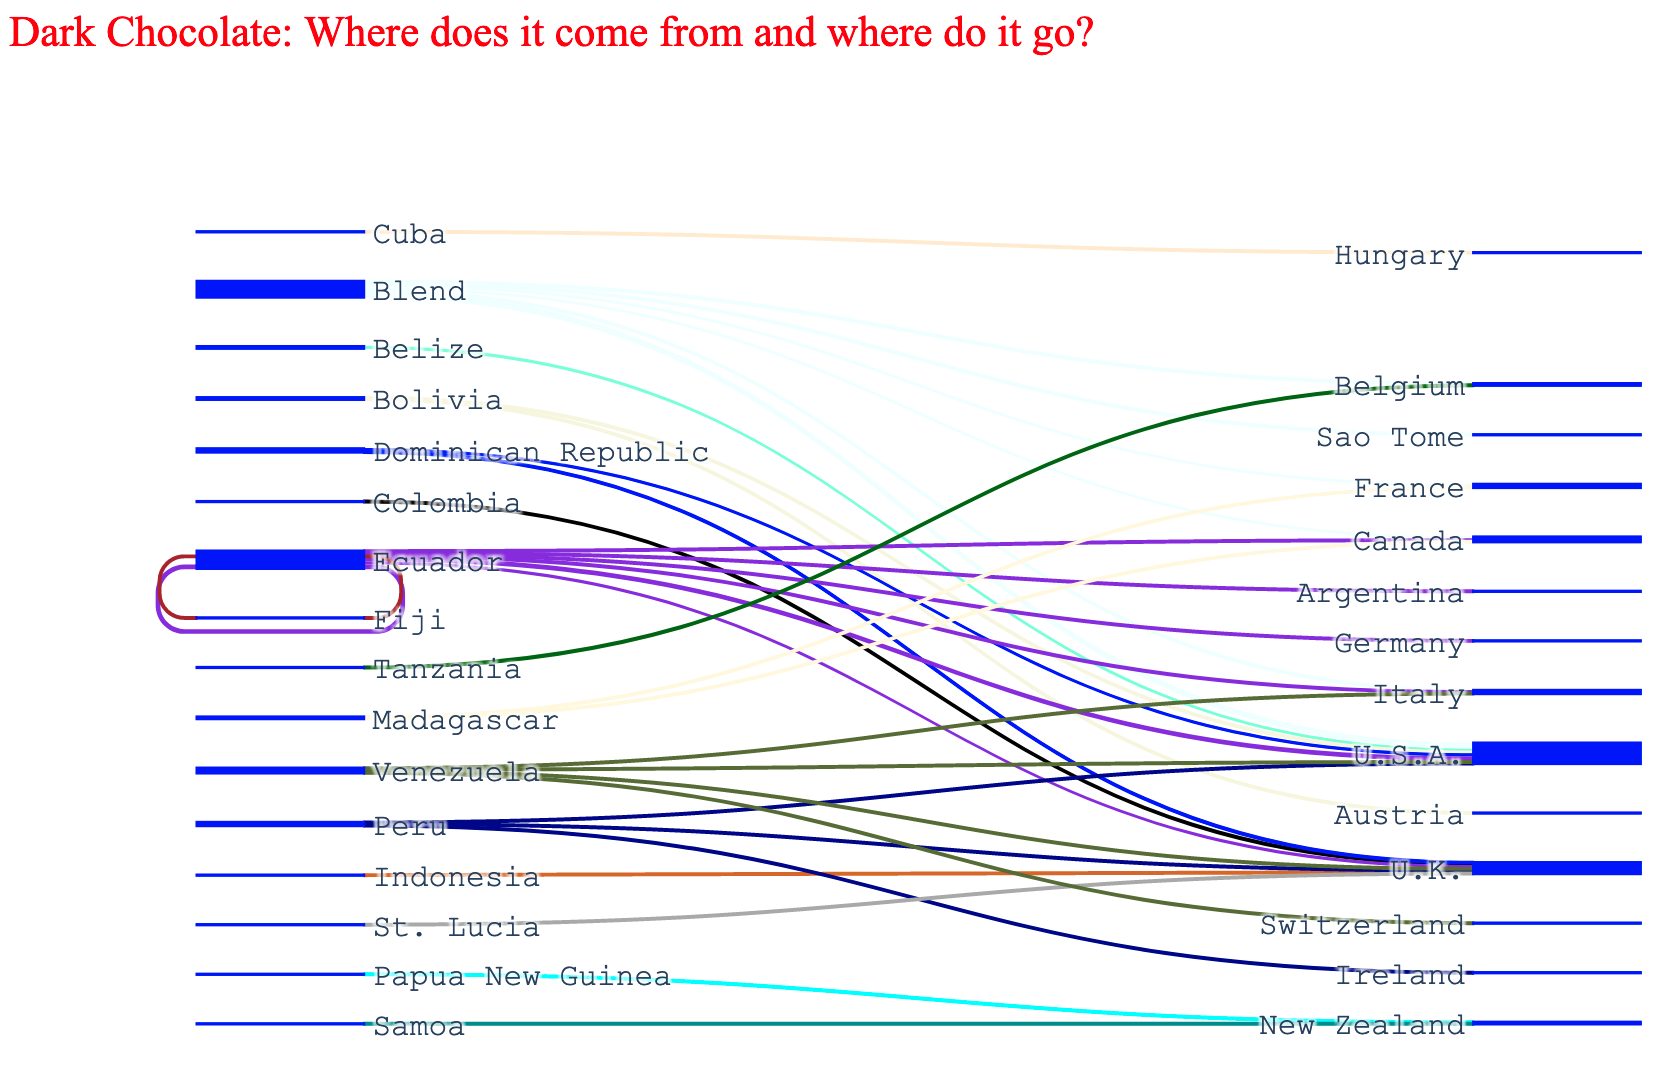
\includegraphics[width=1.0\textwidth]{sankey}
        \caption{Dark Chocolate: Where does it come from and where does it go?}
        \label{fig:sankey}
    \end{figure}
    \item From the visualization, it's clear that the country that exports the most amount of chocolate is "Ecuador" and "Blend". The biggest consumers of dark chocolate are the "U.S.A" and the "UK", followed by "Canada".
    \item Interestingly, we also see some self-loops for "Ecuador" and "Fiji", meaning that they are both the producer and consumer of dark chocolate!
\end{itemize}

\end{document}
